Um die Umsetzbarkeit diese Projektes zu überprüfen, wurde ein Prototyp angefertigt.\\
\\
Aus einem alten Schlauchboot wurde der Boden ausgeschnitten. Danach wurde in einem Holzplatte in der Mitte ein Loch geschnitten und der Motor mit Propeller wurde darüber montiert -- siehe \autoref{fig:ErsterPrototyp}.
\begin{figure}[h!]
  \centering
  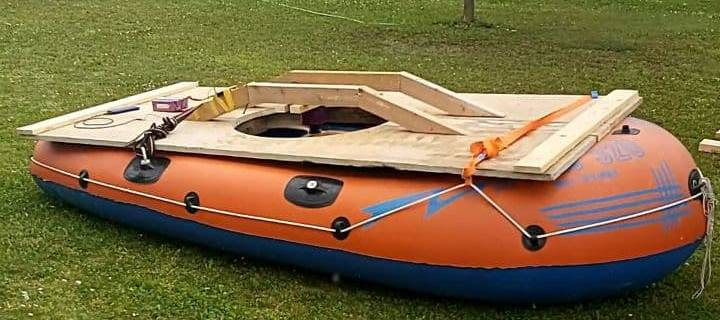
\includegraphics[width=.95\textwidth]{./Aufbau1.jpg}
  \caption{Aufbau erster Prototyp}
  \label{fig:ErsterPrototyp}
\end{figure}

Der Motorregler wurde direkt an zwei in Serie geschaltete 6S-LiPo Akkus angeschlossen und mit einer Fernbedienung gesteuert.\\
Der Test hat gezeigt, dass unser Motor mit dem verwendeten Propeller genug Kraft hat, um einen Menschen zu tragen. Durch die großen Luftspalten zwischen der Holzplatte und dem Schlauchboot geht sehr viel Luft verloren, was die Effizienz stark verschlechtert.

